\section{Nested Free Design and Conditional Expected-Loss Optimization}
\label{sec:nested-design-v13}

The next finite pilot connects two forms of optimization in one original-world
loop. An external designer can change executable institutional source,
mechanisms, protocols, wiring and activity processes. Within each explicitly
authored vocabulary, a conditional sampling distribution can instead be updated
using observed native losses. These are complementary degrees of freedom, not
a claim that arbitrary source generation or the researcher world is
pathwise differentiable.

\paragraph{Prospective objectives and budget.}
The two exact losses are the existing throughput objective $L_A=-A$ and a new
illustrative reviewed-production objective $L_E=-Q+0.5R$. Here $A$ counts native
accepted decisions, $Q$ sums the original integer-parsed reviewer means on
accepted decisions, and $R$ counts actual review records. An unreviewed
acceptance contributes zero to $Q$. Institution-written final scores are not
used. The new coefficient is an explicit engineering preference for review
work, not a calibrated welfare weight or scientific-quality law. It removes
the historical utility objective's per-acceptance cost and increases its
declared review-work cost; it is not a retrospective change to that study.
No additional merit floor, fairness rule, novelty reward or promotion veto is
introduced. The original five authors, two years, seed42, four-year real corpus
and fixed Qwen3:8B weights remain, with no response reuse across worlds.
IID here describes draws from the conditional design distribution, not
independent scientific seeds or researcher-response replications. Every fresh
world resets the same development seed42.

\begin{table}[t]
\caption{The fixed nested schedule is repeated for each objective. Native
attempts total at most eight across both arms; failed slots are not replaced.}
\label{tab:nested-schedule-v13}
\centering
\small
\begin{tabular}{p{.22\linewidth}p{.43\linewidth}p{.23\linewidth}}
\toprule
Stage & Proposal rule & Native attempts / update \\
\midrule
Initial G0 & External complete free vocabulary & Two IID draws; one LR step \\
Updated G0 & Exact G0 vocabulary at saved updated weights & One fresh draw; forward only \\
Redesigned G1 & External complete vocabulary from all own feedback & One fresh draw; forward only \\
\bottomrule
\end{tabular}
\end{table}

\paragraph{What is differentiated.}
For a frozen generated vocabulary $V$, let $d$ denote categorical choices and
unbounded Gaussian latents sampled from its declared distribution
$q_\theta(d\mid V)$. Fixed sigmoids map latents to bounded design coordinates;
source and graph patches map the draw to an executable native system. Subject to
the usual score-function regularity conditions~\citep{parmas2021unified},
\begin{equation}
 \nabla_\theta\mathbb{E}_{d\sim q_\theta,\,\tau\sim\mathrm{Sim}(d)}[L(\tau)]
 =\mathbb{E}[L(\tau)\nabla_\theta\log q_\theta(d\mid V)].
\end{equation}
The simulator, including its language decisions and discrete transitions,
need not expose a Jacobian for this conditional identity. This identity
assumes well-defined integrable costs and a conditional world law
that has no additional dependence on $\theta$ once its full design is given.
An unavailable batch does not identify such a gradient. The implemented
two-draw leave-one-out estimate is
\begin{equation}
 \widehat g=\frac12\bigl[(L_0-L_1)\nabla_\theta\log q_\theta(d_0\mid V)
 +(L_1-L_0)\nabla_\theta\log q_\theta(d_1\mid V)\bigr],
 \qquad \theta^+=\theta-0.1\widehat g.
\end{equation}
Each draw's baseline excludes its own loss. Equal observed costs give zero
advantages; valid empty parameter sets are allowed. Technical failures keep
null losses and leave weights unchanged rather than become fabricated
penalties. The next native draw uses the exact saved $\theta^+$ and G0
vocabulary, with a fresh draw identity. It performs no additional update.
If G0 is valid but the update is unavailable, the scheduled followup uses
unchanged weights. If G0 itself is invalid, that slot is unavailable and
consumed without a replacement world.
This schedules a native followup of the final parameter update rather than
ending immediately after backward. If that attempt fails, its loss stays null
and the updated proposal remains unevaluated; no replacement is inferred.
Neither a noisy step nor one completed followup proves expected improvement.

The external G1 request then exposes all three own preceding observations,
source/graph definitions, failures and the saved update. It preserves every
exact incumbent tie and uses the earliest tie only as a display/parent
representative. G1 may change the algorithms, support and coordinate meanings;
it declares its initial weights explicitly. The host does not silently
transport gradients or control state across incompatible vocabularies.
Retention is legal: useful invention and improving the designer are empirical
questions, not technical acceptance conditions. External Codex authorship
remains self-reported, with request-level own-history instructions rather than
authenticated provider identity or operating-system isolation.

\paragraph{Extending real activities, not replacing the world.}
An opt-in typed review-routing capability exposes the actual submitted papers
and original eligible reviewer identities before review execution. Arbitrary
sandboxed institution source can emit any valid subset of paper/reviewer tasks,
including none. Trusted identity/accounting transport then invokes the original
native prompt, model, integer parser, review record and received-experience
path for those tasks. It does not manufacture scores, charge a new review fee
or provide a reviewer-allocation policy. Existing self/COI eligibility and
duplicate-record legality remain disclosed native semantics, not loss vetoes.
Zero-review systems must explicitly author a compatible admission consumer:
the host does not repair legacy selection or secretly supply missing reviews.
The unchanged default graph retains original behavior when this capability is
absent. This is an additional connection to real work, not a claim that review
is the entire institution or that every possible scientific activity already
has a native consumer.

Prospective research-plan receipts now retain the complete pre-amendment upstream
plan, source port and input-event lineage, in addition to ordered amendment
commands. A read-only auditor can reconstruct the full applied plan and join it
to recorded source outputs and native state, without reexecuting institutional
source or treating provenance as scientific correctness. Historical missing provenance
is not fabricated retroactively. The new audit also independently checks
scalar likelihood derivatives and the single LR update per arm, exact post-update
sampling, checkpoints, actual review tasks and model-request identities.

\paragraph{Inspection and editing boundaries.}
The existing English pixel-art Institution Foundry exposes the nested stages,
before/after distribution weights, source, circuit and recorded plan/review
effects. Its city choreography remains schematic, not measured agent motion.
An observed institution can seed a local editable branch and an explicit
handoff to the existing design workbench. The local draft is never presented
as executed or adopted; runtime validation and renewed compute consent remain
separate. Same-checkpoint cross-scores remain development diagnostics, not
held-out evaluations or extra optimization signals.

\subsection{Actual native results and objective-dependent institutions}

All eight scheduled native worlds complete at clean source \code{fdf4d1c},
using 592 fresh Qwen replies, with no reply reuse or world-level technical
failure (Table~\ref{tab:nested-results-v13}). The independent read-only audit
reextracts every checkpoint loss, replays draws and each arm's single
within-vocabulary update, and joins actual source, wire, task and plan receipts. Two reports are
byte-identical; all 129 raw input files remain unchanged. All 227 replay-critical
source blobs match the actual pin. Forty source executions, 16 complete-plan
effects, 16 routing events and 28 actual review records are verified. These
counts describe native execution, not scientific validity or authenticated
external authorship.

\begin{table}[t]
\caption{All v13 native observations, including worse post-update draws.
Each row is a separate execution at the same development seed, not an
independent seed replication. $L_A=-A$ and $L_E=-Q+0.5R$ are independently
cross-scored on each checkpoint.}
\label{tab:nested-results-v13}
\centering
\small
\begin{tabular}{llrrrrr}
\toprule
Optimized loss & Stage & $A$ & $Q$ & $R$ & $L_A$ & $L_E$ \\
\midrule
Throughput & Initial G0, draw 1 & 7 & 0 & 0 & $-7$ & 0 \\
 & Initial G0, draw 2 & 7 & 0 & 0 & $-7$ & 0 \\
 & Updated G0 & 6 & 0 & 0 & $-6$ & 0 \\
 & Redesigned G1 & 10 & 0 & 0 & $-10$ & 0 \\
\addlinespace[3pt]
Reviewed production & Initial G0, draw 1 & 6 & 20 & 6 & $-6$ & $-17$ \\
 & Initial G0, draw 2 & 6 & 18.5 & 12 & $-6$ & $-12.5$ \\
 & Updated G0 & 6 & 12 & 4 & $-6$ & $-10$ \\
 & Redesigned G1 & 6 & 21 & 6 & $-6$ & $-18$ \\
\bottomrule
\end{tabular}
\end{table}

\paragraph{The conditional update is real, but its followup is not a gain.}
The throughput author's bounded coordinate controls the share of researchers
assigned annual rather than two-year project cycles. Its two initial native
losses tie at $-7$, so the independently checked LOO gradient is exactly zero
and its Gaussian mean remains zero. A fresh draw from that unchanged
distribution has loss $-6$. It is not called an improved gradient proposal.

The reviewed-production author's G0 instead controls review coverage and a
categorical count of zero, one or two reviewers per covered paper. Its
initial losses $[-17,-12.5]$ produce a nonzero update: the coverage latent
mean moves from $1.5$ to $1.671086$ and reviewer-count logits move from
$(-1,1,-1)$ to $(-1,1.225,-1.225)$. The new native draw has loss $-10$, worse
than its first best. A lower-probability or worse sample can follow a valid
distribution update; this single forward neither demonstrates expected-loss
improvement nor invalidates the score identity. Both post-update results and
all exact ties remain in the history passed to G1.

\paragraph{Free source redesign changes the organizing algorithms.}
For throughput, G1 replaces the identity-hashed mixed-cycle algorithm with
universal annual project scheduling, preserving each researcher's native
topic, focus and reason fields while changing project timing. Its coordinate
is removed and its new distribution is explicitly a point mass. The
zero-review dispatcher and compatible all-accept publication rule remain.
Observed count loss improves from the first best $-7$ to $-10$.

For reviewed production, G1 replaces the allocation lottery and rendezvous
ranking with full coverage and one eligible reviewer, ranked by own-history
reviewer scores. The author pools 22 original review records from its three
preceding worlds and shrinks each reviewer's mean with one pooled-mean
pseudo-observation; unseen reviewers receive that pooled mean. A separate
report-only read-only check joins all 22 source records to the three exact
request-bound checkpoints and independently recomputes sums, counts and
ranking. It neither executes source nor becomes a validity or selection veto.
These forecasts select task identities only: actual Qwen reviews and the
original native integer parser still determine $Q$. The new native result
is $Q=21,R=6$, hence $L_E=-18$, better than its first best $-17$.

Both G1 definitions explicitly reset to empty factor/coordinate sets; neither
performs another update or implicitly transports G0 weights. Each changes one
source body, not its topology: the throughput graph stays at 17 nodes/25 wires
and the reviewed-production graph at 16 nodes/23 wires. Their initial free
vocabularies already differ from the shared parent. New labels, hashes or
unchanged graph sizes are not used as evidence of semantic novelty.

\paragraph{What the differences do and do not show.}
The loss-selected systems have same-checkpoint profiles $(L_A,L_E)=(-10,0)$
and $(-6,-18)$ (Figure~\ref{fig:nested-design-v13}). The first exploits a
count proxy through faster cycles without review; the second uses a
review-score proxy to favor reviewers with higher past scores. This observable
proxy-seeking design is a potential metric-gaming route, not evidence of
improved epistemic evaluation or demonstrated harm.
No hidden quality veto is added to remove it. The descriptive development
gains establish executable result-conditioned redesign under two losses, not
causal attribution to a single edit, optimizer superiority, estimator benefit,
generalization, validated scientific value or an endogenously improving
designer. Separate externally authored families and a single development seed
do not identify the objective's causal effect by themselves.

\begin{figure}[p]
\centering
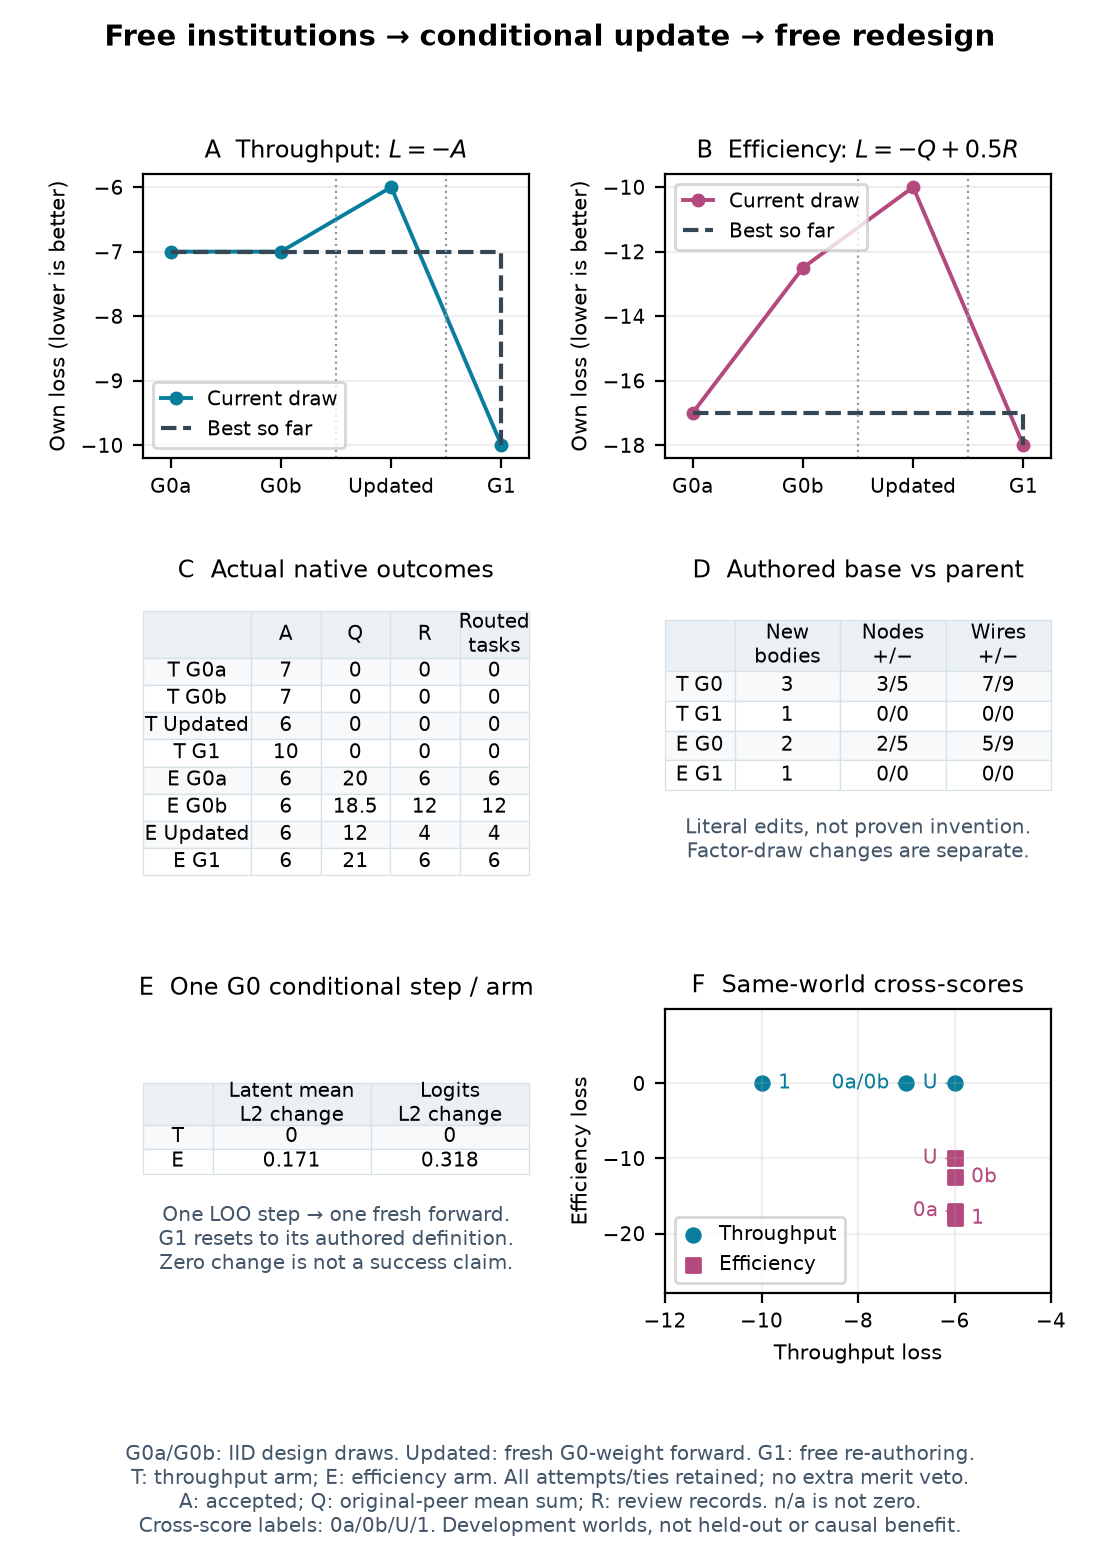
\includegraphics[width=\linewidth]{figures/native-nested-search-v13-a1.png}
\caption{Audited nested optimization paths at native print size. The two
own-loss paths use distinct scales and separate current outcomes from best
so far. Native counts, literal authored edits, each arm's conditional update
and all same-checkpoint cross-scores are retained. Neither post-update draw
beats its prior best; both free G1 code revisions improve their own first
best, without establishing expected or scientific benefit.}
\label{fig:nested-design-v13}
\end{figure}
